
\begin{figure}[!ht]
\centering
\resizebox{\columnwidth}{!}{%\documentclass{standalone}
%
%\usepackage{tikz,pgf} %and any other packages or tikzlibraries your picture needs
%
%\begin{document}
%\resizebox{\columnwidth}{!}{
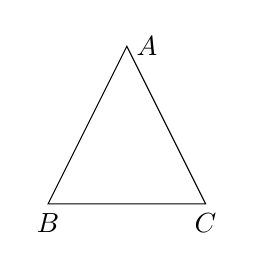
\begin{tikzpicture}
\draw (0,0) node[anchor=north]{$B$}
  -- (1,2) node[anchor=west]{$A$}
  -- (2,0) node[anchor=north]{$C$}
  -- cycle;
\end{tikzpicture}
%}
%\end{document}}
\caption{}
\label{fig:8.1.45_triangle1}	
\end{figure}

\item {\em Construction: } See Fig. \ref{fig:8.1.45_triangle1}.  The input parameters are
\begin{align}
\vec{P} &= \myvec{p\\q},
%\label{eq:constr_a} 
 \vec{Q} &= \myvec{0\\0}, 
\label{eq:constr_b}
\\
\vec{R} &= \myvec{a\\0},
%\label{eq:constr_c}
\label{eq:constr_d}
\end{align}
%
where $\vec{P}$  is obtained by choosing $PR > PQ$.
$\because PS$ is the angle bisector, its equation is given by (see Problem \ref{prob:8.1.23})
%
\begin{align}
PS: \vec{x} = \vec{P} + \lambda\brak{\frac{\vec{P}-\vec{Q}}{\norm{\vec{P}-\vec{Q}}}+\frac{\vec{P}-\vec{R}}{\norm{\vec{P}-\vec{R}}}}
\end{align}
%
$\vec{S}$ is obtained as the intersection of $PS$ and $QR$.


